% Options for packages loaded elsewhere
\PassOptionsToPackage{unicode}{hyperref}
\PassOptionsToPackage{hyphens}{url}
%
\documentclass[
]{article}
\usepackage{lmodern}
\usepackage{amssymb,amsmath}
\usepackage{ifxetex,ifluatex}
\ifnum 0\ifxetex 1\fi\ifluatex 1\fi=0 % if pdftex
  \usepackage[T1]{fontenc}
  \usepackage[utf8]{inputenc}
  \usepackage{textcomp} % provide euro and other symbols
\else % if luatex or xetex
  \usepackage{unicode-math}
  \defaultfontfeatures{Scale=MatchLowercase}
  \defaultfontfeatures[\rmfamily]{Ligatures=TeX,Scale=1}
\fi
% Use upquote if available, for straight quotes in verbatim environments
\IfFileExists{upquote.sty}{\usepackage{upquote}}{}
\IfFileExists{microtype.sty}{% use microtype if available
  \usepackage[]{microtype}
  \UseMicrotypeSet[protrusion]{basicmath} % disable protrusion for tt fonts
}{}
\makeatletter
\@ifundefined{KOMAClassName}{% if non-KOMA class
  \IfFileExists{parskip.sty}{%
    \usepackage{parskip}
  }{% else
    \setlength{\parindent}{0pt}
    \setlength{\parskip}{6pt plus 2pt minus 1pt}}
}{% if KOMA class
  \KOMAoptions{parskip=half}}
\makeatother
\usepackage{xcolor}
\IfFileExists{xurl.sty}{\usepackage{xurl}}{} % add URL line breaks if available
\IfFileExists{bookmark.sty}{\usepackage{bookmark}}{\usepackage{hyperref}}
\hypersetup{
  pdftitle={RMarkdown en 10 minutos},
  pdfauthor={Mauricio Bucca},
  hidelinks,
  pdfcreator={LaTeX via pandoc}}
\urlstyle{same} % disable monospaced font for URLs
\usepackage[margin=1in]{geometry}
\usepackage{color}
\usepackage{fancyvrb}
\newcommand{\VerbBar}{|}
\newcommand{\VERB}{\Verb[commandchars=\\\{\}]}
\DefineVerbatimEnvironment{Highlighting}{Verbatim}{commandchars=\\\{\}}
% Add ',fontsize=\small' for more characters per line
\usepackage{framed}
\definecolor{shadecolor}{RGB}{248,248,248}
\newenvironment{Shaded}{\begin{snugshade}}{\end{snugshade}}
\newcommand{\AlertTok}[1]{\textcolor[rgb]{0.94,0.16,0.16}{#1}}
\newcommand{\AnnotationTok}[1]{\textcolor[rgb]{0.56,0.35,0.01}{\textbf{\textit{#1}}}}
\newcommand{\AttributeTok}[1]{\textcolor[rgb]{0.77,0.63,0.00}{#1}}
\newcommand{\BaseNTok}[1]{\textcolor[rgb]{0.00,0.00,0.81}{#1}}
\newcommand{\BuiltInTok}[1]{#1}
\newcommand{\CharTok}[1]{\textcolor[rgb]{0.31,0.60,0.02}{#1}}
\newcommand{\CommentTok}[1]{\textcolor[rgb]{0.56,0.35,0.01}{\textit{#1}}}
\newcommand{\CommentVarTok}[1]{\textcolor[rgb]{0.56,0.35,0.01}{\textbf{\textit{#1}}}}
\newcommand{\ConstantTok}[1]{\textcolor[rgb]{0.00,0.00,0.00}{#1}}
\newcommand{\ControlFlowTok}[1]{\textcolor[rgb]{0.13,0.29,0.53}{\textbf{#1}}}
\newcommand{\DataTypeTok}[1]{\textcolor[rgb]{0.13,0.29,0.53}{#1}}
\newcommand{\DecValTok}[1]{\textcolor[rgb]{0.00,0.00,0.81}{#1}}
\newcommand{\DocumentationTok}[1]{\textcolor[rgb]{0.56,0.35,0.01}{\textbf{\textit{#1}}}}
\newcommand{\ErrorTok}[1]{\textcolor[rgb]{0.64,0.00,0.00}{\textbf{#1}}}
\newcommand{\ExtensionTok}[1]{#1}
\newcommand{\FloatTok}[1]{\textcolor[rgb]{0.00,0.00,0.81}{#1}}
\newcommand{\FunctionTok}[1]{\textcolor[rgb]{0.00,0.00,0.00}{#1}}
\newcommand{\ImportTok}[1]{#1}
\newcommand{\InformationTok}[1]{\textcolor[rgb]{0.56,0.35,0.01}{\textbf{\textit{#1}}}}
\newcommand{\KeywordTok}[1]{\textcolor[rgb]{0.13,0.29,0.53}{\textbf{#1}}}
\newcommand{\NormalTok}[1]{#1}
\newcommand{\OperatorTok}[1]{\textcolor[rgb]{0.81,0.36,0.00}{\textbf{#1}}}
\newcommand{\OtherTok}[1]{\textcolor[rgb]{0.56,0.35,0.01}{#1}}
\newcommand{\PreprocessorTok}[1]{\textcolor[rgb]{0.56,0.35,0.01}{\textit{#1}}}
\newcommand{\RegionMarkerTok}[1]{#1}
\newcommand{\SpecialCharTok}[1]{\textcolor[rgb]{0.00,0.00,0.00}{#1}}
\newcommand{\SpecialStringTok}[1]{\textcolor[rgb]{0.31,0.60,0.02}{#1}}
\newcommand{\StringTok}[1]{\textcolor[rgb]{0.31,0.60,0.02}{#1}}
\newcommand{\VariableTok}[1]{\textcolor[rgb]{0.00,0.00,0.00}{#1}}
\newcommand{\VerbatimStringTok}[1]{\textcolor[rgb]{0.31,0.60,0.02}{#1}}
\newcommand{\WarningTok}[1]{\textcolor[rgb]{0.56,0.35,0.01}{\textbf{\textit{#1}}}}
\usepackage{longtable,booktabs}
% Correct order of tables after \paragraph or \subparagraph
\usepackage{etoolbox}
\makeatletter
\patchcmd\longtable{\par}{\if@noskipsec\mbox{}\fi\par}{}{}
\makeatother
% Allow footnotes in longtable head/foot
\IfFileExists{footnotehyper.sty}{\usepackage{footnotehyper}}{\usepackage{footnote}}
\makesavenoteenv{longtable}
\usepackage{graphicx,grffile}
\makeatletter
\def\maxwidth{\ifdim\Gin@nat@width>\linewidth\linewidth\else\Gin@nat@width\fi}
\def\maxheight{\ifdim\Gin@nat@height>\textheight\textheight\else\Gin@nat@height\fi}
\makeatother
% Scale images if necessary, so that they will not overflow the page
% margins by default, and it is still possible to overwrite the defaults
% using explicit options in \includegraphics[width, height, ...]{}
\setkeys{Gin}{width=\maxwidth,height=\maxheight,keepaspectratio}
% Set default figure placement to htbp
\makeatletter
\def\fps@figure{htbp}
\makeatother
\setlength{\emergencystretch}{3em} % prevent overfull lines
\providecommand{\tightlist}{%
  \setlength{\itemsep}{0pt}\setlength{\parskip}{0pt}}
\setcounter{secnumdepth}{-\maxdimen} % remove section numbering

\title{RMarkdown en 10 minutos}
\author{Mauricio Bucca}
\date{Agosto de 2020}

\begin{document}
\maketitle

\hypertarget{primeros-pasos}{%
\subsection{Primeros pasos}\label{primeros-pasos}}

\begin{figure}
\centering
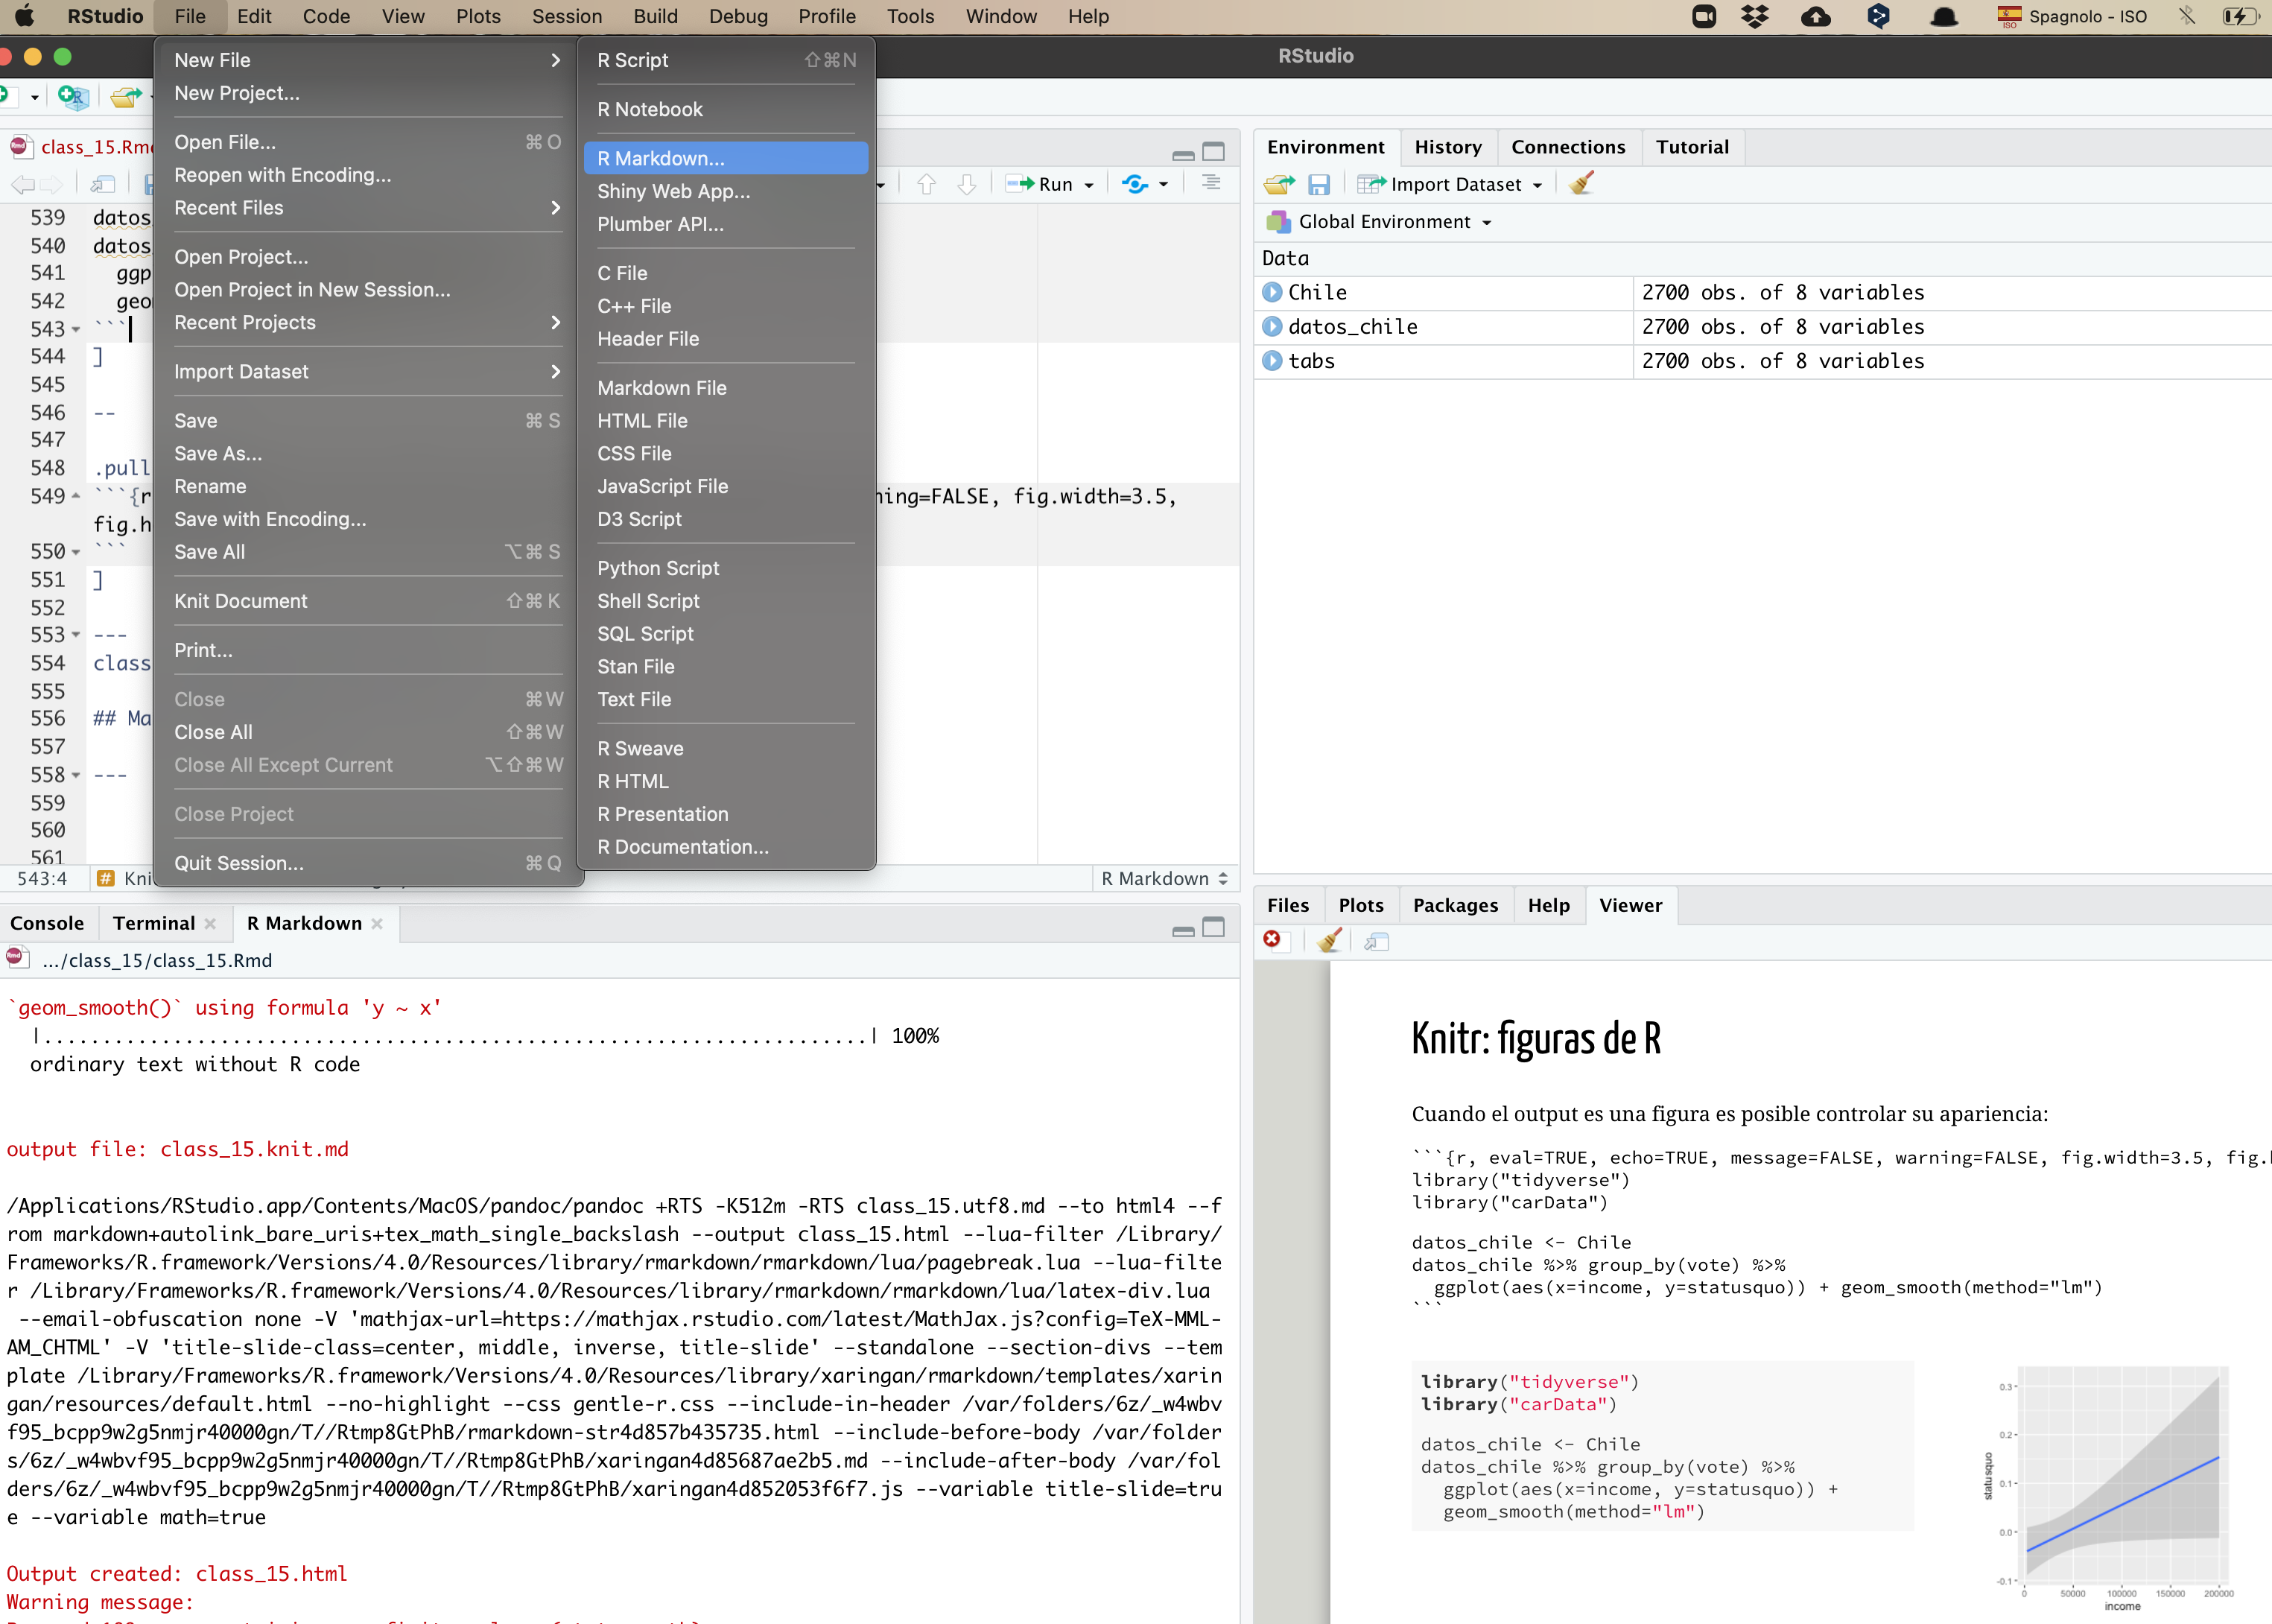
\includegraphics{images/inicio.png}
\caption{Newfile}
\end{figure}

\hypertarget{introducciuxf3n}{%
\subsection{Introducción}\label{introducciuxf3n}}

\hypertarget{texto}{%
\subsection{Texto}\label{texto}}

La parte principal de un informe en \texttt{RMarkdown} suele ser texto.
En un fichero .Rmd, todo lo que no sea encabezamiento código será
interpretado como texto y lo mostrará tal cual. El texto de un documento
\texttt{.Rmd} es ``simplemente'' texto PERO está escrito en
\emph{Markdown}. Lo que escribamos en Rmarkdown se mostrará tal cual en
el documento final, pero es posible dar un poco de formato: negritas,
cursivas, listas, enlaces de internet, etc\ldots{}

Para mayor detalle:
\href{https://www.markdownguide.org/cheat-sheet/}{aquí}

\hypertarget{ecuaciones}{%
\subsection{Ecuaciones}\label{ecuaciones}}

En \texttt{Rmarkdown} se pueden introducir formulas matemáticas
(escritas en \texttt{Látex}). Para formulas en linea se usa el signo
\texttt{\$} al inicio y al final de la expresión. Por ejemplo, el código
\texttt{\$y\_\{i\}\ =\ \textbackslash{}alpha\ +\ \textbackslash{}beta\_\{1\}x\_\{i\}\ +\ \textbackslash{}beta\_\{2\}x\^{}\{2\}\_\{i\}\ +\ \textbackslash{}epsilon\_\{i\}\$}
produce la siguiente ecuación:
\(y_{i} = \alpha + \beta_{1}x_{i} \beta_{2}x^{2}_{i} + \epsilon_{i}\).

Para escribir la misma ecuación en una linea independiente, se usa el
signo \texttt{\$\$}. Por ejemplo, el código
\texttt{\$\$y\_\{i\}\ =\ \textbackslash{}alpha\ +\ \textbackslash{}beta\_\{1\}x\_\{i\}\ +\ \textbackslash{}beta\_\{2\}x\^{}\{2\}\_\{i\}\ +\ \textbackslash{}epsilon\_\{i\}\$\$}
produce la siguiente ecuación:

\[y_{i} = \alpha + \beta_{1}x_{i} + \beta_{2}x^{2}_{i} + \epsilon_{i}\]

Para mayor detalle:
\href{https://en.wikibooks.org/wiki/LaTeX/Mathematics}{aquí}

\hypertarget{cuxf3digo-chunks}{%
\subsection{Código (``chunks'')}\label{cuxf3digo-chunks}}

\texttt{RMarkdown} permite introducir código de \texttt{R} en el
documento de texto, evaluar tal código y mostrar los resultados
directamente en el informe. A modo de ejemplo, comenzaremos mostrando un
\texttt{summary} de la base de datos \texttt{iris}, que viene incluida
en \texttt{R}.

\begin{Shaded}
\begin{Highlighting}[]
\KeywordTok{summary}\NormalTok{(iris)}
\end{Highlighting}
\end{Shaded}

\begin{verbatim}
##   Sepal.Length    Sepal.Width     Petal.Length    Petal.Width          Species  
##  Min.   :4.300   Min.   :2.000   Min.   :1.000   Min.   :0.100   setosa    :50  
##  1st Qu.:5.100   1st Qu.:2.800   1st Qu.:1.600   1st Qu.:0.300   versicolor:50  
##  Median :5.800   Median :3.000   Median :4.350   Median :1.300   virginica :50  
##  Mean   :5.843   Mean   :3.057   Mean   :3.758   Mean   :1.199                  
##  3rd Qu.:6.400   3rd Qu.:3.300   3rd Qu.:5.100   3rd Qu.:1.800                  
##  Max.   :7.900   Max.   :4.400   Max.   :6.900   Max.   :2.500
\end{verbatim}

El trozo de arriba es un chunk de código \texttt{R}. Al compilar el
documento, (click en el botón \texttt{knitr}, en el panel) el código se
ejecutará y mostrarán los resultados en el documento final. Los chunks
pueden tienen diversas opciones que permiten una mayor flexibilidad en
como se muestra el código y los resultados. Las opciones más usadas son:

\begin{itemize}
\tightlist
\item
  echo
\item
  eval
\end{itemize}

Por ejemplo, el chunk abajo mostrará el código (\texttt{echo\ =\ TRUE}),
lo evaluará y mostrará los resultados en el documento final
(\texttt{eval\ =\ TRUE}). Así se ve:

\begin{Shaded}
\begin{Highlighting}[]
\NormalTok{a <-}\StringTok{ }\KeywordTok{summary}\NormalTok{(iris)}
\KeywordTok{print}\NormalTok{(a)}
\end{Highlighting}
\end{Shaded}

\begin{verbatim}
##   Sepal.Length    Sepal.Width     Petal.Length    Petal.Width          Species  
##  Min.   :4.300   Min.   :2.000   Min.   :1.000   Min.   :0.100   setosa    :50  
##  1st Qu.:5.100   1st Qu.:2.800   1st Qu.:1.600   1st Qu.:0.300   versicolor:50  
##  Median :5.800   Median :3.000   Median :4.350   Median :1.300   virginica :50  
##  Mean   :5.843   Mean   :3.057   Mean   :3.758   Mean   :1.199                  
##  3rd Qu.:6.400   3rd Qu.:3.300   3rd Qu.:5.100   3rd Qu.:1.800                  
##  Max.   :7.900   Max.   :4.400   Max.   :6.900   Max.   :2.500
\end{verbatim}

Si sólo queremos mostrar el código (\texttt{echo\ =\ TRUE}) pero no
evaluarlo (\texttt{eval\ =\ FALSE}), escribimos lo siguiente:

\begin{Shaded}
\begin{Highlighting}[]
\NormalTok{a <-}\StringTok{ }\KeywordTok{summary}\NormalTok{(iris)}
\KeywordTok{print}\NormalTok{(a)}
\end{Highlighting}
\end{Shaded}

Por el contrario, si queremos evaluar el código, mostrar sus resultados,
pero no mostrar el código mismo, escribimos:

\begin{verbatim}
##   Sepal.Length    Sepal.Width     Petal.Length    Petal.Width          Species  
##  Min.   :4.300   Min.   :2.000   Min.   :1.000   Min.   :0.100   setosa    :50  
##  1st Qu.:5.100   1st Qu.:2.800   1st Qu.:1.600   1st Qu.:0.300   versicolor:50  
##  Median :5.800   Median :3.000   Median :4.350   Median :1.300   virginica :50  
##  Mean   :5.843   Mean   :3.057   Mean   :3.758   Mean   :1.199                  
##  3rd Qu.:6.400   3rd Qu.:3.300   3rd Qu.:5.100   3rd Qu.:1.800                  
##  Max.   :7.900   Max.   :4.400   Max.   :6.900   Max.   :2.500
\end{verbatim}

Por último, si queremos NO mostrar el código (\texttt{echo\ =\ FALSE}),
SI evaluarlo (\texttt{eval\ =\ FALSE}), PERO NO se mostrar los
resultados (\texttt{results\ =\ "hide"}), escribimos:

Que el código haya sido evaluado significa que el objeto ``a'' existirá
en la memoria y podrá ser usado para posterior análisis.

\hypertarget{gruxe1ficos}{%
\subsection{Gráficos}\label{gruxe1ficos}}

También podemos mostrar gráficos producidos en \texttt{R}. Notar que los
paquetes necesarios para implementar un determinado análisis
(\texttt{ggplot2} y \texttt{tidyverse}, en este caso) deben ser
previamente cargados.

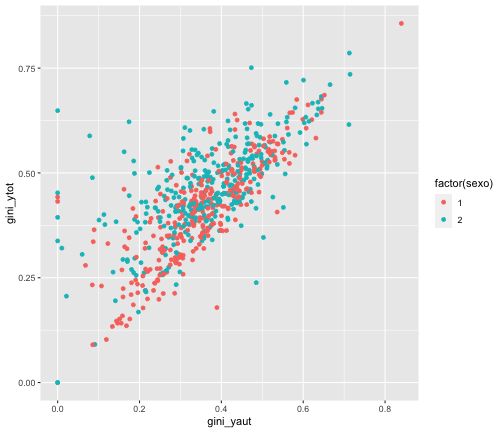
\includegraphics{class_15_template_files/figure-latex/unnamed-chunk-6-1.pdf}

Para eliminar el mensaje entregado por R usamos la opción
\texttt{message=FALSE}:

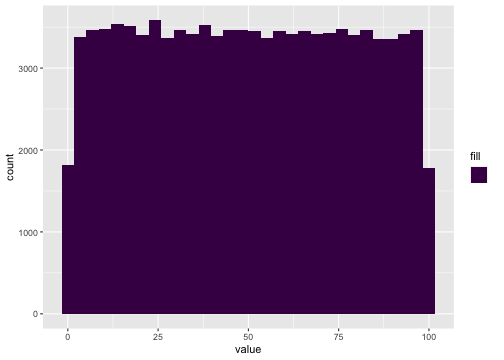
\includegraphics{class_15_template_files/figure-latex/unnamed-chunk-7-1.pdf}

\hypertarget{tablas}{%
\subsection{Tablas}\label{tablas}}

Este reporte usa datos de la base de datos \texttt{iris}:

\begin{longtable}[]{@{}rrrrl@{}}
\toprule
Sepal.Length & Sepal.Width & Petal.Length & Petal.Width &
Species\tabularnewline
\midrule
\endhead
5.1 & 3.5 & 1.4 & 0.2 & setosa\tabularnewline
4.9 & 3.0 & 1.4 & 0.2 & setosa\tabularnewline
4.7 & 3.2 & 1.3 & 0.2 & setosa\tabularnewline
4.6 & 3.1 & 1.5 & 0.2 & setosa\tabularnewline
5.0 & 3.6 & 1.4 & 0.2 & setosa\tabularnewline
5.4 & 3.9 & 1.7 & 0.4 & setosa\tabularnewline
4.6 & 3.4 & 1.4 & 0.3 & setosa\tabularnewline
5.0 & 3.4 & 1.5 & 0.2 & setosa\tabularnewline
4.4 & 2.9 & 1.4 & 0.2 & setosa\tabularnewline
4.9 & 3.1 & 1.5 & 0.1 & setosa\tabularnewline
5.4 & 3.7 & 1.5 & 0.2 & setosa\tabularnewline
4.8 & 3.4 & 1.6 & 0.2 & setosa\tabularnewline
4.8 & 3.0 & 1.4 & 0.1 & setosa\tabularnewline
4.3 & 3.0 & 1.1 & 0.1 & setosa\tabularnewline
5.8 & 4.0 & 1.2 & 0.2 & setosa\tabularnewline
5.7 & 4.4 & 1.5 & 0.4 & setosa\tabularnewline
5.4 & 3.9 & 1.3 & 0.4 & setosa\tabularnewline
5.1 & 3.5 & 1.4 & 0.3 & setosa\tabularnewline
5.7 & 3.8 & 1.7 & 0.3 & setosa\tabularnewline
5.1 & 3.8 & 1.5 & 0.3 & setosa\tabularnewline
5.4 & 3.4 & 1.7 & 0.2 & setosa\tabularnewline
5.1 & 3.7 & 1.5 & 0.4 & setosa\tabularnewline
4.6 & 3.6 & 1.0 & 0.2 & setosa\tabularnewline
5.1 & 3.3 & 1.7 & 0.5 & setosa\tabularnewline
4.8 & 3.4 & 1.9 & 0.2 & setosa\tabularnewline
5.0 & 3.0 & 1.6 & 0.2 & setosa\tabularnewline
5.0 & 3.4 & 1.6 & 0.4 & setosa\tabularnewline
5.2 & 3.5 & 1.5 & 0.2 & setosa\tabularnewline
5.2 & 3.4 & 1.4 & 0.2 & setosa\tabularnewline
4.7 & 3.2 & 1.6 & 0.2 & setosa\tabularnewline
4.8 & 3.1 & 1.6 & 0.2 & setosa\tabularnewline
5.4 & 3.4 & 1.5 & 0.4 & setosa\tabularnewline
5.2 & 4.1 & 1.5 & 0.1 & setosa\tabularnewline
5.5 & 4.2 & 1.4 & 0.2 & setosa\tabularnewline
4.9 & 3.1 & 1.5 & 0.2 & setosa\tabularnewline
5.0 & 3.2 & 1.2 & 0.2 & setosa\tabularnewline
5.5 & 3.5 & 1.3 & 0.2 & setosa\tabularnewline
4.9 & 3.6 & 1.4 & 0.1 & setosa\tabularnewline
4.4 & 3.0 & 1.3 & 0.2 & setosa\tabularnewline
5.1 & 3.4 & 1.5 & 0.2 & setosa\tabularnewline
5.0 & 3.5 & 1.3 & 0.3 & setosa\tabularnewline
4.5 & 2.3 & 1.3 & 0.3 & setosa\tabularnewline
4.4 & 3.2 & 1.3 & 0.2 & setosa\tabularnewline
5.0 & 3.5 & 1.6 & 0.6 & setosa\tabularnewline
5.1 & 3.8 & 1.9 & 0.4 & setosa\tabularnewline
4.8 & 3.0 & 1.4 & 0.3 & setosa\tabularnewline
5.1 & 3.8 & 1.6 & 0.2 & setosa\tabularnewline
4.6 & 3.2 & 1.4 & 0.2 & setosa\tabularnewline
5.3 & 3.7 & 1.5 & 0.2 & setosa\tabularnewline
5.0 & 3.3 & 1.4 & 0.2 & setosa\tabularnewline
7.0 & 3.2 & 4.7 & 1.4 & versicolor\tabularnewline
6.4 & 3.2 & 4.5 & 1.5 & versicolor\tabularnewline
6.9 & 3.1 & 4.9 & 1.5 & versicolor\tabularnewline
5.5 & 2.3 & 4.0 & 1.3 & versicolor\tabularnewline
6.5 & 2.8 & 4.6 & 1.5 & versicolor\tabularnewline
5.7 & 2.8 & 4.5 & 1.3 & versicolor\tabularnewline
6.3 & 3.3 & 4.7 & 1.6 & versicolor\tabularnewline
4.9 & 2.4 & 3.3 & 1.0 & versicolor\tabularnewline
6.6 & 2.9 & 4.6 & 1.3 & versicolor\tabularnewline
5.2 & 2.7 & 3.9 & 1.4 & versicolor\tabularnewline
5.0 & 2.0 & 3.5 & 1.0 & versicolor\tabularnewline
5.9 & 3.0 & 4.2 & 1.5 & versicolor\tabularnewline
6.0 & 2.2 & 4.0 & 1.0 & versicolor\tabularnewline
6.1 & 2.9 & 4.7 & 1.4 & versicolor\tabularnewline
5.6 & 2.9 & 3.6 & 1.3 & versicolor\tabularnewline
6.7 & 3.1 & 4.4 & 1.4 & versicolor\tabularnewline
5.6 & 3.0 & 4.5 & 1.5 & versicolor\tabularnewline
5.8 & 2.7 & 4.1 & 1.0 & versicolor\tabularnewline
6.2 & 2.2 & 4.5 & 1.5 & versicolor\tabularnewline
5.6 & 2.5 & 3.9 & 1.1 & versicolor\tabularnewline
5.9 & 3.2 & 4.8 & 1.8 & versicolor\tabularnewline
6.1 & 2.8 & 4.0 & 1.3 & versicolor\tabularnewline
6.3 & 2.5 & 4.9 & 1.5 & versicolor\tabularnewline
6.1 & 2.8 & 4.7 & 1.2 & versicolor\tabularnewline
6.4 & 2.9 & 4.3 & 1.3 & versicolor\tabularnewline
6.6 & 3.0 & 4.4 & 1.4 & versicolor\tabularnewline
6.8 & 2.8 & 4.8 & 1.4 & versicolor\tabularnewline
6.7 & 3.0 & 5.0 & 1.7 & versicolor\tabularnewline
6.0 & 2.9 & 4.5 & 1.5 & versicolor\tabularnewline
5.7 & 2.6 & 3.5 & 1.0 & versicolor\tabularnewline
5.5 & 2.4 & 3.8 & 1.1 & versicolor\tabularnewline
5.5 & 2.4 & 3.7 & 1.0 & versicolor\tabularnewline
5.8 & 2.7 & 3.9 & 1.2 & versicolor\tabularnewline
6.0 & 2.7 & 5.1 & 1.6 & versicolor\tabularnewline
5.4 & 3.0 & 4.5 & 1.5 & versicolor\tabularnewline
6.0 & 3.4 & 4.5 & 1.6 & versicolor\tabularnewline
6.7 & 3.1 & 4.7 & 1.5 & versicolor\tabularnewline
6.3 & 2.3 & 4.4 & 1.3 & versicolor\tabularnewline
5.6 & 3.0 & 4.1 & 1.3 & versicolor\tabularnewline
5.5 & 2.5 & 4.0 & 1.3 & versicolor\tabularnewline
5.5 & 2.6 & 4.4 & 1.2 & versicolor\tabularnewline
6.1 & 3.0 & 4.6 & 1.4 & versicolor\tabularnewline
5.8 & 2.6 & 4.0 & 1.2 & versicolor\tabularnewline
5.0 & 2.3 & 3.3 & 1.0 & versicolor\tabularnewline
5.6 & 2.7 & 4.2 & 1.3 & versicolor\tabularnewline
5.7 & 3.0 & 4.2 & 1.2 & versicolor\tabularnewline
5.7 & 2.9 & 4.2 & 1.3 & versicolor\tabularnewline
6.2 & 2.9 & 4.3 & 1.3 & versicolor\tabularnewline
5.1 & 2.5 & 3.0 & 1.1 & versicolor\tabularnewline
5.7 & 2.8 & 4.1 & 1.3 & versicolor\tabularnewline
6.3 & 3.3 & 6.0 & 2.5 & virginica\tabularnewline
5.8 & 2.7 & 5.1 & 1.9 & virginica\tabularnewline
7.1 & 3.0 & 5.9 & 2.1 & virginica\tabularnewline
6.3 & 2.9 & 5.6 & 1.8 & virginica\tabularnewline
6.5 & 3.0 & 5.8 & 2.2 & virginica\tabularnewline
7.6 & 3.0 & 6.6 & 2.1 & virginica\tabularnewline
4.9 & 2.5 & 4.5 & 1.7 & virginica\tabularnewline
7.3 & 2.9 & 6.3 & 1.8 & virginica\tabularnewline
6.7 & 2.5 & 5.8 & 1.8 & virginica\tabularnewline
7.2 & 3.6 & 6.1 & 2.5 & virginica\tabularnewline
6.5 & 3.2 & 5.1 & 2.0 & virginica\tabularnewline
6.4 & 2.7 & 5.3 & 1.9 & virginica\tabularnewline
6.8 & 3.0 & 5.5 & 2.1 & virginica\tabularnewline
5.7 & 2.5 & 5.0 & 2.0 & virginica\tabularnewline
5.8 & 2.8 & 5.1 & 2.4 & virginica\tabularnewline
6.4 & 3.2 & 5.3 & 2.3 & virginica\tabularnewline
6.5 & 3.0 & 5.5 & 1.8 & virginica\tabularnewline
7.7 & 3.8 & 6.7 & 2.2 & virginica\tabularnewline
7.7 & 2.6 & 6.9 & 2.3 & virginica\tabularnewline
6.0 & 2.2 & 5.0 & 1.5 & virginica\tabularnewline
6.9 & 3.2 & 5.7 & 2.3 & virginica\tabularnewline
5.6 & 2.8 & 4.9 & 2.0 & virginica\tabularnewline
7.7 & 2.8 & 6.7 & 2.0 & virginica\tabularnewline
6.3 & 2.7 & 4.9 & 1.8 & virginica\tabularnewline
6.7 & 3.3 & 5.7 & 2.1 & virginica\tabularnewline
7.2 & 3.2 & 6.0 & 1.8 & virginica\tabularnewline
6.2 & 2.8 & 4.8 & 1.8 & virginica\tabularnewline
6.1 & 3.0 & 4.9 & 1.8 & virginica\tabularnewline
6.4 & 2.8 & 5.6 & 2.1 & virginica\tabularnewline
7.2 & 3.0 & 5.8 & 1.6 & virginica\tabularnewline
7.4 & 2.8 & 6.1 & 1.9 & virginica\tabularnewline
7.9 & 3.8 & 6.4 & 2.0 & virginica\tabularnewline
6.4 & 2.8 & 5.6 & 2.2 & virginica\tabularnewline
6.3 & 2.8 & 5.1 & 1.5 & virginica\tabularnewline
6.1 & 2.6 & 5.6 & 1.4 & virginica\tabularnewline
7.7 & 3.0 & 6.1 & 2.3 & virginica\tabularnewline
6.3 & 3.4 & 5.6 & 2.4 & virginica\tabularnewline
6.4 & 3.1 & 5.5 & 1.8 & virginica\tabularnewline
6.0 & 3.0 & 4.8 & 1.8 & virginica\tabularnewline
6.9 & 3.1 & 5.4 & 2.1 & virginica\tabularnewline
6.7 & 3.1 & 5.6 & 2.4 & virginica\tabularnewline
6.9 & 3.1 & 5.1 & 2.3 & virginica\tabularnewline
5.8 & 2.7 & 5.1 & 1.9 & virginica\tabularnewline
6.8 & 3.2 & 5.9 & 2.3 & virginica\tabularnewline
6.7 & 3.3 & 5.7 & 2.5 & virginica\tabularnewline
6.7 & 3.0 & 5.2 & 2.3 & virginica\tabularnewline
6.3 & 2.5 & 5.0 & 1.9 & virginica\tabularnewline
6.5 & 3.0 & 5.2 & 2.0 & virginica\tabularnewline
6.2 & 3.4 & 5.4 & 2.3 & virginica\tabularnewline
5.9 & 3.0 & 5.1 & 1.8 & virginica\tabularnewline
\bottomrule
\end{longtable}

\end{document}
